\documentclass[12pt,a4paper]{exam}
\usepackage[paperwidth=9cm,paperheight=16cm,left=0.7cm,right=0.7cm,bottom=2cm,top=2cm]{geometry}
\usepackage{jdlm}
\title{\vspace{-2.2cm}\textsc{Elasticity}}
\author{Practice Problems\\November 2019}
\runningheader{\textit{Elasticity Practice Problems}}{}{}
\footer{}{}{\vspace{-1.5cm}\includegraphics[scale=0.15]{../feathers-logo.png}}
\date{}
\setlength{\columnseprule}{0.4pt}
\newcommand{\Lim}[2]{\lim\limits_{#1 \rightarrow #2}}
%\color{white}
\definecolor{taupe}{rgb}{0.28, 0.24, 0.2}
%\pagecolor{taupe}
%\color{white}
\begin{document}
		%\pagecolor{taupe}
		\begin{center}
			\vspace{-3cm}\textsc{Physics: Elasticity}\\
			Practice Problems\\ \vspace{0.1cm}
			\tiny{November 2019}
		\end{center}

\begin{questions}
	\question Two wires of the same material and length are stretched
	by the same force. Their masses are in the ratio $3 : 2$, their
	elongations are in the ratio :
	\begin{choices}
		\choice		$3:2$
		\choice		$9:4$
		\choice		$2:3$
		\choice		$4:9$
	\end{choices}
	
	\question	A cable that can support a load of 800 N is cut into two
	equal parts. The maximum load that can be supported
	by either part is :
	\begin{choices}
		\choice		100 N
		\choice		400 N
		\choice		800 N
		\choice		1600 N
	\end{choices}

	\question		When a weight of 5 kg is suspended from a copper wire of length 30 m and radius 0.5 mm, the length of the wire
	increases by 2.4 cm. If the radius is doubled, the extension
	produced is:
	\begin{choices}
		\choice		1.2 cm
		\choice		0.6 cm
		\choice		0.3 cm
		\choice		0.15 cm
	\end{choices}

	\question		The Young's modulus of steel is twice that of brass. Two wires of same length and of same area of cross-section, one of steel and the other of brass, are suspended from the same roof. If we want the lower ends of the wires to be at the same level, then the weights  added to the steel and brass wires must be in the ratio:
	\begin{choices}
		\choice		$4:1$
		\choice		$1:1$
		\choice		$1:2$
		\choice		$2:1$
	\end{choices}
	
	\question		If the ratio of diameters, lengths and Young's modulii of steel and copper wires shown in the figure are $p,q$ and $s$ respectively, then the corresponding ratio of increase in their lengths would be
	\begin{figure}[!htb]
		\centering
		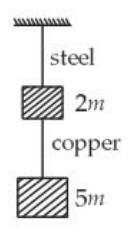
\includegraphics[scale=0.5]{Y-st-br.png}
	\end{figure}
	\begin{choices}
		\choice		$\dfrac{5q}{7sp^2}$
		\choice		$\dfrac{7q}{5sp^2}$
		\choice		$\dfrac{2q}{5sp}$
		\choice		$\dfrac{7q}{5sp}$
	\end{choices}
	
	\question		For a constant hydraulic stress on an object, the fractional change in volume $ (\Delta V / V) $ and its bulk modulus $ (B) $ are related as 
	\begin{choices}
		\choice		$\dfrac{\Delta V}{V} \propto B$
		\choice		$\dfrac{\Delta V}{V} \propto \dfrac{1}{B}$
		\choice		$\dfrac{\Delta V}{V} \propto B^2$
		\choice		$\dfrac{\Delta V}{V} \propto \dfrac{1}{B^2}$
	\end{choices}
	
	\question		For a constant hydraulic stress $ P $ on an object with bulk modulus $ B $, the fractional change in the volume will be \\
	\begin{choices}
		\choice		$ \dfrac{P}{B} $
		\choice		$ \dfrac{B}{P} $
		\choice		$ \sqrt{\dfrac{P}{B}} $
		\choice		$ \left(\dfrac{B}{P}\right)^2 $
	\end{choices}

\question	A cube is subjected to a uniform volume compression. If the side of the cube decreases by $ 2\% $, the bulk strain is:
\begin{choices}
	\choice		0.02
	\choice		0.03
	\choice		0.04
	\choice		0.06
\end{choices}

\question	In question 7, the fractional change in radius is:
\begin{choices}
	\choice		$ \dfrac{B}{3P} $
	\choice		$ \dfrac{3P}{B} $
	\choice		$ \dfrac{P}{3B} $
	\choice		$ \dfrac{P}{B} $
\end{choices}
	
\end{questions}

\end{document}
